\documentclass[
10pt,
a4paper,
oneside,
headinclude,footinclude,
BCOR5mm,
]{scrartcl}

%%%%%%%%%%%%%%%%%%%%%%%%%%%%%%%%%%%%%%%%%
% Arsclassica Article
% Structure Specification File
%
% This file has been downloaded from:
% http://www.LaTeXTemplates.com
%
% Original author:
% Lorenzo Pantieri (http://www.lorenzopantieri.net) with extensive modifications by:
% Vel (vel@latextemplates.com)
%
% License:
% CC BY-NC-SA 3.0 (http://creativecommons.org/licenses/by-nc-sa/3.0/)
%
%%%%%%%%%%%%%%%%%%%%%%%%%%%%%%%%%%%%%%%%%

%----------------------------------------------------------------------------------------
%	REQUIRED PACKAGES
%----------------------------------------------------------------------------------------

\usepackage[
nochapters, % Turn off chapters since this is an article        
beramono, % Use the Bera Mono font for monospaced text (\texttt)
eulermath,% Use the Euler font for mathematics
pdfspacing, % Makes use of pdftex’ letter spacing capabilities via the microtype package
dottedtoc % Dotted lines leading to the page numbers in the table of contents
]{classicthesis} % The layout is based on the Classic Thesis style

\usepackage{arsclassica} % Modifies the Classic Thesis package

\usepackage[T1]{fontenc} % Use 8-bit encoding that has 256 glyphs

\usepackage[utf8]{inputenc} % Required for including letters with accents

\usepackage{graphicx} % Required for including images
\graphicspath{{Figures/}} % Set the default folder for images

\usepackage{enumitem} % Required for manipulating the whitespace between and within lists

\usepackage{lipsum} % Used for inserting dummy 'Lorem ipsum' text into the template

\usepackage{subfig} % Required for creating figures with multiple parts (subfigures)

\usepackage{amsmath,amssymb,amsthm} % For including math equations, theorems, symbols, etc

\usepackage{varioref} % More descriptive referencing

%----------------------------------------------------------------------------------------
%	THEOREM STYLES
%---------------------------------------------------------------------------------------

\theoremstyle{definition} % Define theorem styles here based on the definition style (used for definitions and examples)
\newtheorem{definition}{Definition}

\theoremstyle{plain} % Define theorem styles here based on the plain style (used for theorems, lemmas, propositions)
\newtheorem{theorem}{Theorem}

\theoremstyle{remark} % Define theorem styles here based on the remark style (used for remarks and notes)

%----------------------------------------------------------------------------------------
%	HYPERLINKS
%---------------------------------------------------------------------------------------

\hypersetup{
%draft, % Uncomment to remove all links (useful for printing in black and white)
colorlinks=true, breaklinks=true, bookmarks=true,bookmarksnumbered,
urlcolor=webbrown, linkcolor=RoyalBlue, citecolor=webgreen, % Link colors
pdftitle={}, % PDF title
pdfauthor={\textcopyright}, % PDF Author
pdfsubject={}, % PDF Subject
pdfkeywords={}, % PDF Keywords
pdfcreator={pdfLaTeX}, % PDF Creator
pdfproducer={LaTeX with hyperref and ClassicThesis} % PDF producer
}

\hyphenation{Fortran hy-phen-ation}

\title{\normalfont\spacedallcaps{Osclass Latch Plugin User Manual}}
\author{\spacedlowsmallcaps{Daniel Esteban}}

\begin{document}

\renewcommand{\sectionmark}[1]{\markright{\spacedlowsmallcaps{#1}}}
\lehead{\mbox{\llap{\small\thepage\kern1em\color{halfgray} \vline}\color{halfgray}\hspace{0.5em}\rightmark\hfil}}

\pagestyle{scrheadings} 

\maketitle
\setcounter{tocdepth}{2}
\tableofcontents
\listoffigures

\section*{Abstract}
User manual for Osclass Latch plugin that allows you to use Latch services in your Osclass installation for both, regular users and administratos.


\newpage 

\section{About this plugin}
The purpose of this plugin is to offer extra security to both, users and administrators, of any website made with Osclass software. Allowing users and administrators to protect and avoid their accounts being accessed without their consent. This plugin was originally made by \href{https://github.com/conejoninja}{Daniel Esteban} and its code is hosted at \href{https://github.com/conejoninja/osclass-latch}{https://github.com/conejoninja/osclass-latch}. It could be downloaded too from Osclass' market \href{http://market.osclass.org/plugins/user-managment/latch\_129}{http://market.osclass.org/plugins/user-managment/latch\_129}. It is distributed under Apache License v2.0, the reader could obtain a copy of it from \href{http://www.apache.org/licenses/LICENSE-2.0}{http://www.apache.org/licenses/LICENSE-2.0}.


\section{Pre-requisites}
Basic knowledge about Osclass and Latch is required as it's not the purpose of this guide to explain how Osclass or Latch is installed, configured or work. It will be assumed that the reader have a working installation of Osclass in a server with the ability to make API calls to the Latch servers (CURL or fsock functions enabled in PHP). It will be assumed too that the reader has a Latch developer account with at least one application created. For more detailed information about how to install and configure Osclass please visit \href{http://doc.osclass.org/}{http://doc.osclass.org/}. For information about Latch and how to create a developer account visit \href{https://latch.elevenpaths.com/}{https://latch.elevenpaths.com/}.

\section{What is Latch?}

\textbf{Latch} (\href{https://latch.elevenpaths.com/}{https://latch.elevenpaths.com/}) is a service that lets you add an extra level of security to your online services. To help prevent any unauthorized use, Latch gives you the control to switch off your accounts with a single tap when you’re not using them. \\
\\
\textit{Security and Control with a single tap}.




\section{Installation}
There are three methods to install this plugin in your Osclass website.

\subsection{Osclass' market}
The easiest way to install this plugin is to access the market from your admin panel (figure ~\ref{fig:market} on page~\pageref{fig:market}), then search for the plugin and download it(figure ~\ref{fig:download} on page~\pageref{fig:download}). Go to your admin panel > Manage plugins and click \textit{Install} on the plugin. See the following video of the installation \href{https://www.youtube.com/watch?v=clKTpgew-Lo}{https://www.youtube.com/watch?v=clKTpgew-Lo}.



\begin{figure}[h!]
  \begin{center}
    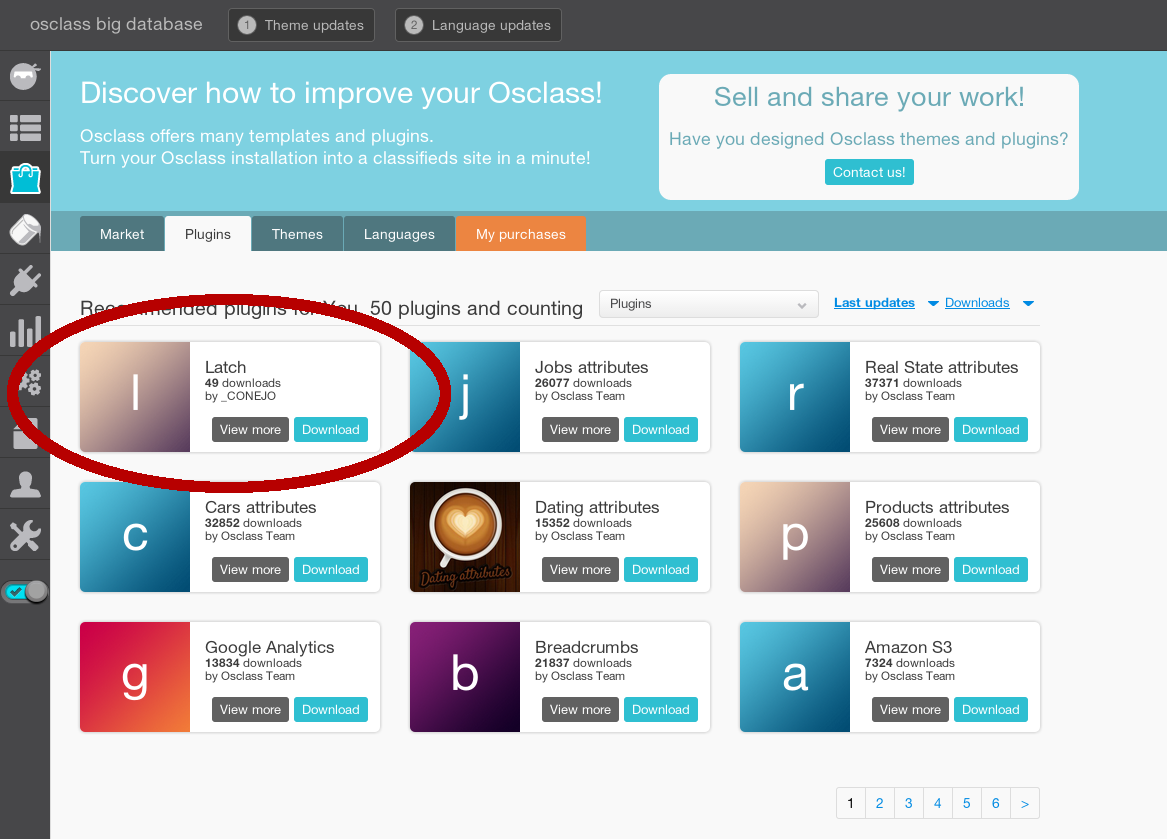
\includegraphics[width=.45\columnwidth]{1}
    \caption{Market area in admin panel}
    \label{fig:market}
  \end{center}
\end{figure}



\begin{figure}[h!]
  \begin{center}
    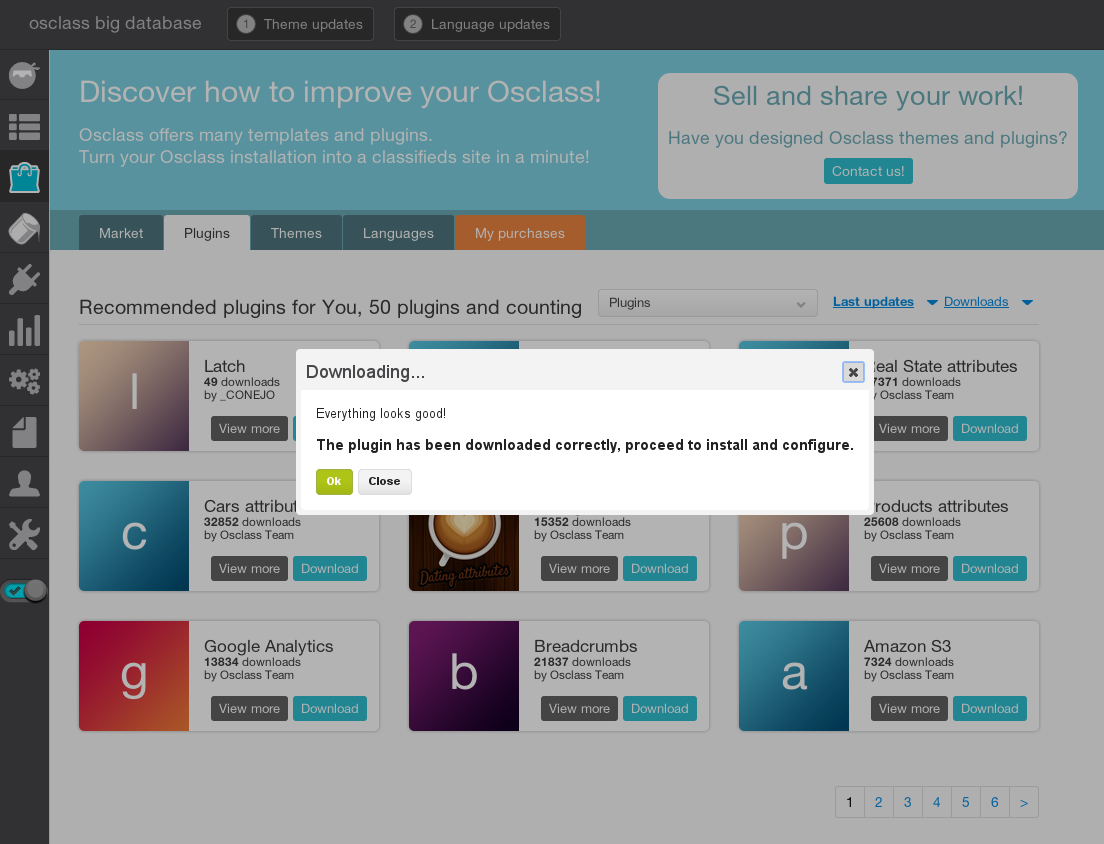
\includegraphics[width=.45\columnwidth]{2}
    \caption{Downloading the Latch plugin}
    \label{fig:download}
  \end{center}
\end{figure}


\subsection{Zip file}
Download the zip file from the market. Go to your admin panel >  Manage plugins, click on the + symbol (add plugin), choose the zip file in the form and click upload. Go to your admin panel > Manage plugins and click \textit{Install} on the plugin.

\subsection{Manual upload}
Download the zip file from the market. Unzip the file on your computer, upload \textit{latch} folder to your sever at \textit{oc-content/plugins/} with your favourite FTP Client. Go to your admin panel > Manage plugins and click \textit{Install} on the plugin.


\section{Configuration}
Access your developer account at \href{https://latch.elevenpaths.com/www/}{https://latch.elevenpaths.com/www/} (if you don't have one, go create a developer accout now). You need to create an application on \textit{Latch}'s website, you could find detailed information on how to create one there. Once the application is created, write down its \textit{appId} and \textit{appSecret}. Go to your \textit{admin panel > Plugins > Configure Latch plugin}. Input your \textit{appId} and \textit{appSecret} and click save. Your plugin is now configured. As seen in figure ~\ref{fig:configuration} on page~\pageref{fig:configuration}.



\begin{figure}[h!]
  \begin{center}
    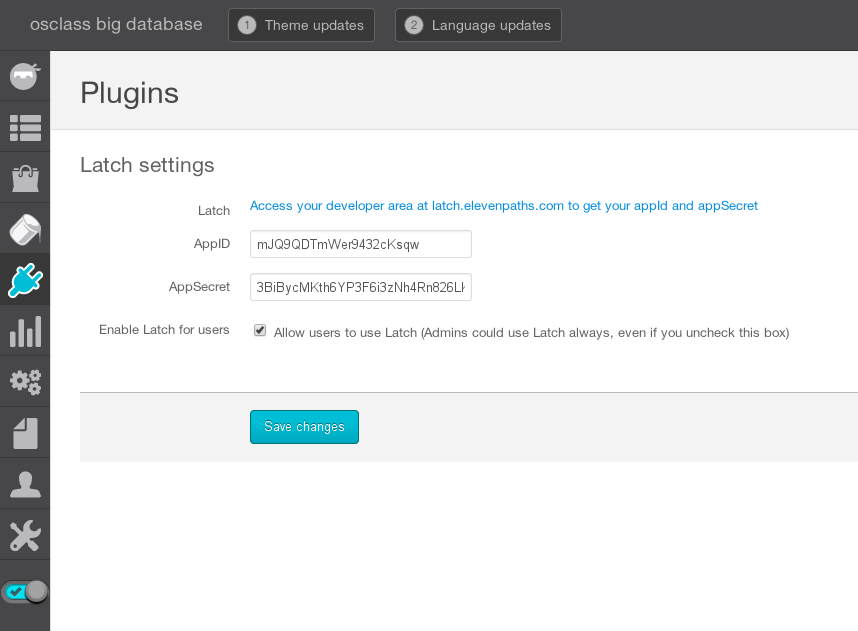
\includegraphics[width=.45\columnwidth]{3}
    \caption{Configuration of Latch plugin}
    \label{fig:configuration}
  \end{center}
\end{figure}


\section{Usage}
\subsection{Users}
Users will find an optional input field for a \textit{Latch}'s pairing code at registration process or when editing their own profile as shown in figure ~\ref{fig:user} on page~\pageref{fig:user}. If the \textit{Latch}'s pairing code is wrong, it will display the proper error on submit, as well as a success message if the pairing is done properly. Once an account is paired, instead of an input field, it will display a link to unpair it.  See the following video for an example of pairing and use for regular users \href{https://www.youtube.com/watch?v=fSsSRi2HuFE}{https://www.youtube.com/watch?v=fSsSRi2HuFE}


\begin{figure}[h!]
  \begin{center}
    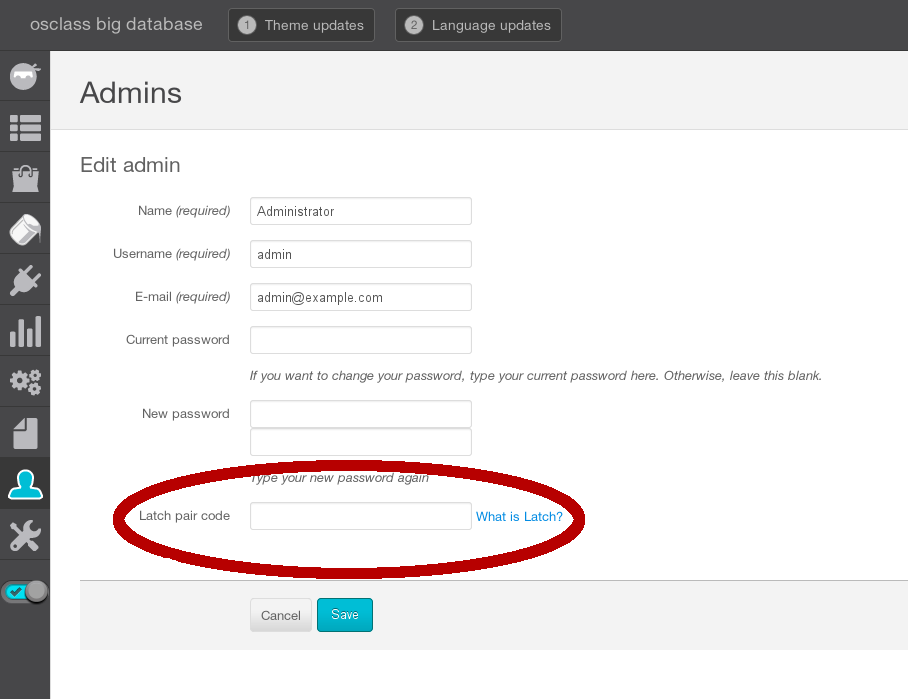
\includegraphics[width=.45\columnwidth]{4}
    \caption{Pairing Latch at user profile}
    \label{fig:user}
  \end{center}
\end{figure}


\subsection{Administrators}
Similar to what regular users will experience, administrators will find an optional input field for a \textit{Latch}'s pairing code when editing their own profile, as shown in figure ~\ref{fig:admin} on page~\pageref{fig:admin}. If the \textit{Latch}'s pairing code is wrong, it will display the proper error on submit, as well as a success message if the pairing is done properly. Once an account is paired, instead of an input field, it will display a link to unpair it. See the following video for an example of pairing and use for administrators \href{https://www.youtube.com/watch?v=QdXFjRXv87w}{https://www.youtube.com/watch?v=QdXFjRXv87w}.



\begin{figure}[h!]
  \begin{center}
    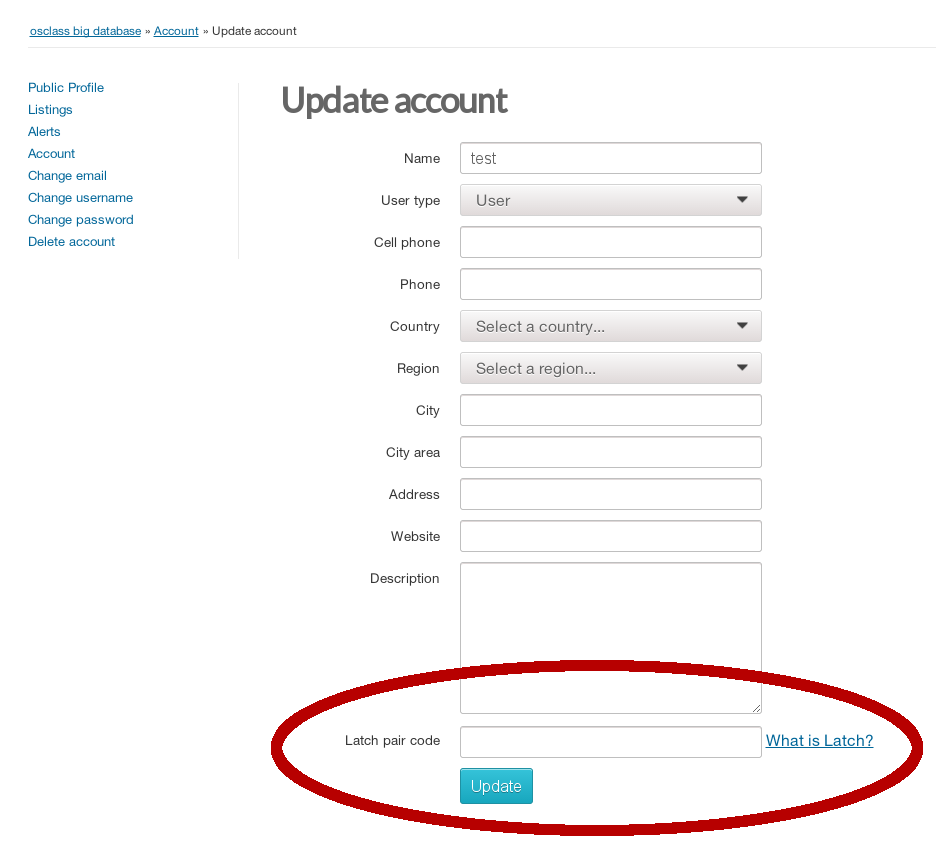
\includegraphics[width=.45\columnwidth]{5}
    \caption{Pairing Latch at admin profile}
    \label{fig:admin}
  \end{center}
\end{figure}

\section{Uninstallation}
If for some reason you want to stop using the plugin, go to your admin panel >  Manage plugins and click on the uninstall link. This action will unpair all current paired accounts and uninstall the plugin from your Osclass website. Be aware that users will have to re-pair with their accounts if you decided to use the plugin again. If you only want to temporarily stop using the plugin, you could disable it from the Manage plugins area in your admin panel. This action will disable the plugin (will not check if the Latch is locked or not) but will not remove any information. If enabled again, your users will be able to continue using their already paired accounts.


\end{document}
